\documentclass{article}
\usepackage{spconf,amsmath,amssymb,graphicx,booktabs}
\usepackage{float,balance}
\usepackage{fontspec}
\setmainfont{texgyretermes-regular.otf}[
    BoldFont=texgyretermes-bold.otf,
    ItalicFont=texgyretermes-italic.otf,
    BoldItalicFont=texgyretermes-bolditalic.otf]
\setsansfont{texgyreheros-regular.otf}[
    BoldFont=texgyreheros-bold.otf,
    ItalicFont=texgyreheros-italic.otf,
    BoldItalicFont=texgyreheros-bolditalic.otf]
\setmonofont{texgyrecursor-regular.otf}[
    BoldFont=texgyrecursor-bold.otf,
    ItalicFont=texgyrecursor-italic.otf,
    BoldItalicFont=texgyrecursor-bolditalic.otf]
\usepackage{hyperref}
\hypersetup{
    hidelinks,
    pdftitle={Receiver-Induced Moment Exchange for Distributed LMB Fusion},
    pdfauthor={Jinhao Chen, Hao Lang, Tianyu Wo},
    pdfkeywords={distributed multi-object tracking, labeled random finite sets, LMB filter, geometric-average fusion, communication-efficient distributed tracking}}
\setcounter{dbltopnumber}{1}
\newcommand{\confsectionstar}[1]{%
    \par\medskip
    {\centering\bfseries\MakeUppercase{#1}\par}
    \smallskip}

\title{Receiver-Induced Moment Exchange for Distributed LMB Fusion}

\name{Jinhao Chen$^{1}$, Hao Lang$^{2,3}$, Tianyu Wo$^{1}$\sthanks{Corresponding author: Tianyu Wo (woty@buaa.edu.cn).}}
\address{$^{1}$Beihang University, Beijing, China\\
$^{2}$Shanghai Jiao Tong University, Shanghai, China\\
$^{3}$Chinese Aeronautical Radio Electronics Research Institute, Shanghai, China}

\begin{document}
\maketitle

\begin{abstract}
Distributed labeled multi-Bernoulli (LMB) trackers can transmit full Gaussian-mixture (GM) messages even when a receiver first collapses each label to one Gaussian. We audit a custom presence-conditioned geometric-average LMB receiver and derive its wire representation from this first irreversible map. Moment matching itself is standard; the contribution is an executable interface certificate spanning label presence, source weighting, deterministic regularization, and serialization. Under the stated admissible numerical contract, sender-side projection preserves every receiver-observable field. A versioned binary codec realizes the interface. In 50 paired eight-sensor trials, moment exchange reduced attempted application-layer payload by 58.28\% (95\% bootstrap interval: 57.92--58.64\%). All 1,119,037 audited retained post-step label instances matched exactly. More generally, the result suggests deriving messages from a receiver's first irreversible map; exactness here remains limited to this receiver and does not extend to mixture-aware or multi-round consumers.
\end{abstract}

\begin{keywords}
Distributed multi-object tracking, labeled random finite sets, LMB filter, geometric-average fusion, communication-efficient distributed tracking
\end{keywords}

\section{Introduction}
\label{sec:introduction}

Distributed multi-object tracking combines complementary sensor views without
centralizing measurements. Labeled multi-Bernoulli (LMB) filters jointly
represent target existence, state uncertainty, and identity
\cite{Vo2014LRFS,Reuter2014LMB,Vo2019MSGLMB}. A Gaussian-mixture (GM) LMB
message may contain several components per label. The studied implementation
serializes every component although its receiver immediately collapses each
label to one Gaussian. It therefore transmits fields this receiver cannot
observe.

Communication-aware RFS trackers reduce transmission frequency, select mixture
components, or exchange projected state estimates
\cite{Shen2022EventTriggeredLMB,Li2023EventTriggeredConsensusLMB,
Shen2024IntegralEventLMB,
Li2019PartialConsensusGMPHD,Xue2026StateCovProjection}. These methods decide
when to send, which components to share, or which compact estimate to form. We
instead ask a consumer-facing question: for a fixed receiver, which transmitted
fields can affect its output?

We study a projected Gaussian KLA-LMB receiver with one synchronous neighbor-
fusion round per filtering step. It aligns labels, normalizes Metropolis weights
over sources carrying each label, projects each GM Bernoulli to existence and
two moments, and fuses the resulting Gaussians. Let $\mathcal T$ denote the
canonical encode/decode content map. For the executed receiver
$\mathcal F_{\omega,\mathcal R}=\mathcal G_{\omega,\mathcal R}\circ\mathcal P$,
the wire-path identity is
$\mathcal F_{\omega,\mathcal R}(\mathcal T\pi)=
\mathcal F_{\omega,\mathcal R}(\mathcal T\mathcal P\pi)$. The nontrivial check
is that label presence, Gaussian overlap, and deterministic regularization also
factor through $\mathcal P$ after transport
(Fig.~\ref{fig:receiver-factorization}).

Our contributions are threefold. First, we extract an executable receiver
contract that includes label presence, KLA weights, covariance canonicalization,
and solve regularization. Second, a versioned application-layer codec and
adversarial property tests validate the contract across serialization. Third, a
frozen 50-trial paired evaluation shows a 58.28\% mean attempted-byte reduction
and zero residual across 1,119,037 label-instance comparisons. We claim neither
equality of the underlying mixture densities nor sufficiency for a mixture-aware
or multi-round receiver.

\begin{figure*}[t]
    \centering
    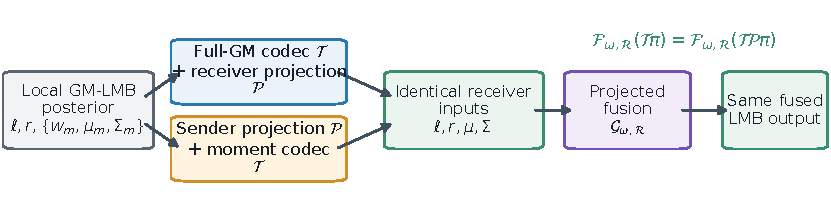
\includegraphics[width=0.94\textwidth]{figures/payload_graph_schematic.pdf}
    \caption{Receiver-induced message factorization. The full path encodes the GM and projects after decoding; the moment path projects before value-preserving encoding. Under Proposition~1's contract, both paths present identical fields to $\mathcal G_{\omega,\mathcal R}$ and produce the same LMB output.}
    \label{fig:receiver-factorization}
\end{figure*}
\begin{figure*}[t]
    \centering
    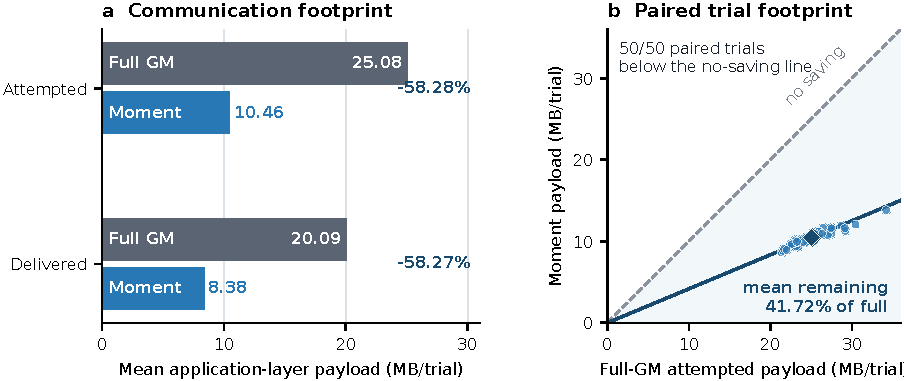
\includegraphics[width=0.94\textwidth]{figures/heldout_tradeoff.pdf}
    \caption{Communication evidence from 50 paired trials. Left: mean attempted and delivered application-layer payloads; percentages are mean per-trial reductions. Right: each point is one paired trial; all lie below the no-saving identity. The retained-field audit is reported in Sec.~\ref{sec:experiments}.}
    \label{fig:confirmatory-evidence}
\end{figure*}
\section{Related Work}
\label{sec:related-work}

Random finite-set filters model uncertain cardinality and association. PHD
filtering gives a first-moment recursion \cite{Mahler2003PHD}; labeled RFS/LMB
models retain identity \cite{Vo2014LRFS,Reuter2014LMB}, and multi-sensor variants
support cooperation \cite{Vo2019MSGLMB}. Under unknown cross-correlations,
KLA/GCI forms a normalized geometric mean \cite{Battistelli2014KLA}, with PHD
and multi-Bernoulli RFS formulations \cite{Uney2013EMDPHD,Wang2017MBGCI}.
Consensus and robust LMB/LRFS methods address networked tracking, including
label-set inconsistency
\cite{Fantacci2015ConsensusLRFS,Shen2022ConsensusLMB,
Li2018RobustDistributedLRFS,Li2019EfficientMultiAgentLRFS}. Minimum-information-
loss and arithmetic-average LMB rules instead use different density-level
objectives \cite{Gao2020MIL,Wei2024AALMB}. These works determine how labeled
posteriors are fused. We propose no new density-level rule and audit only the
custom presence-conditioned per-label update defined below.

\newpage

Communication methods alter a different layer. Event-triggered LMB methods
change when updates are transmitted
\cite{Shen2022EventTriggeredLMB,Li2023EventTriggeredConsensusLMB}; related
triggers act on $M\delta$-GLMB labels or hypotheses
\cite{Li2026EventTriggeredMdeltaGLMB}. Partial-consensus PHD changes which GM
components are disseminated \cite{Li2019PartialConsensusGMPHD}. State and
covariance projection constructs compact track-level inputs for asynchronous
Gaussian fusion \cite{Xue2026StateCovProjection}. In contrast, we hold the
fusion rule, schedule, selection, and receiver fixed, then derive the message
from that receiver's first projection. The certificate covers label/existence,
Gaussian overlap, missing-label normalization, and the codec. Triggering could
be composed with this interface, but that combination is not evaluated here.

\section{Fusion-Sufficient Moment Exchange}
\label{sec:method}

\subsection{Label-Wise Moment Projection}

At time $k$, source $j$ maintains an LMB posterior
\begin{equation}
\begin{split}
    \pi_j &= \{(r_j^\ell,p_j^\ell):\ell\in\mathcal L_j\},\\
    p_j^\ell(x)&=\sum_{m=1}^{M_j^\ell}w_{jm}^\ell
    \mathcal N(x;m_{jm}^\ell,P_{jm}^\ell).
\end{split}
    \label{eq:lmb-gm}
\end{equation}
For normalized $w_{jm}^\ell$, define the label-wise projection $\mathcal P$ by
\begin{equation}
 \mathcal P(\pi_j)=\{(r_j^\ell,\mathcal N(\mu_j^\ell,\Sigma_j^\ell))\}_\ell,
 \quad \mu_j^\ell=\sum_m w_{jm}^\ell m_{jm}^\ell,
 \label{eq:projection}
\end{equation}
\begin{equation}
 \Sigma_j^\ell=\sum_m w_{jm}^\ell\!\left[P_{jm}^\ell+
 (m_{jm}^\ell-\mu_j^\ell)(m_{jm}^\ell-\mu_j^\ell)^\top\right].
 \label{eq:covariance}
\end{equation}
This keeps the label and existence probability and replaces the mixture by the
Gaussian with identical first two moments. The projection is idempotent:
$\mathcal P(\mathcal P(\pi))=\mathcal P(\pi)$.

\subsection{The Projected Gaussian KLA-LMB Receiver}

Receiver $i$ first applies $\mathcal P$ to every delivered source, aligns the
union of labels, and then fuses one Gaussian per label. Let
$\mathcal S_i^\ell$ contain self and delivered neighbors carrying label
$\ell$. Let $\alpha_{ij}$ and $\beta_{ij}$ be the spatial and existence
weights. Missing-label renormalization gives
\begin{equation}
 a_{ij}^\ell=\frac{\alpha_{ij}}{\sum_{q\in\mathcal S_i^\ell}\alpha_{iq}},
 \qquad
 b_{ij}^\ell=\frac{\beta_{ij}}{\sum_{q\in\mathcal S_i^\ell}\beta_{iq}}.
 \label{eq:active-weights}
\end{equation}
The Gaussian canonical parameters are
\begin{equation}
\begin{split}
 K_i^\ell&=\sum_{j\in\mathcal S_i^\ell}a_{ij}^\ell(\Sigma_j^\ell)^{-1},
 \quad h_i^\ell=\sum_j a_{ij}^\ell(\Sigma_j^\ell)^{-1}\mu_j^\ell,\\
 \bar\Sigma_i^\ell&=(K_i^\ell)^{-1},\qquad
 \bar\mu_i^\ell=\bar\Sigma_i^\ell h_i^\ell.
\end{split}
 \label{eq:gaussian-fusion}
\end{equation}
Define the Gaussian overlap by
\begin{equation}
\begin{split}
 \eta_i^\ell&=\int \varphi_i^\ell(x)\,dx,\\
 \varphi_i^\ell(x)&=\prod_{j\in\mathcal S_i^\ell}
 \mathcal N(x;\mu_j^\ell,\Sigma_j^\ell)^{a_{ij}^\ell}.
\end{split}
 \label{eq:gaussian-overlap}
\end{equation}
The Bernoulli terms are
\begin{equation}
 q_1^\ell=\eta_i^\ell\prod_j(r_j^\ell)^{b_{ij}^\ell},\quad
 q_0^\ell=\prod_j(1-r_j^\ell)^{b_{ij}^\ell},\quad
 \bar r_i^\ell=\frac{q_1^\ell}{q_0^\ell+q_1^\ell}.
 \label{eq:existence-fusion}
\end{equation}
where all products in Eq.~\eqref{eq:existence-fusion} are over
$j\in\mathcal S_i^\ell$.
The implementation clamps each $r_j^\ell$ to $[10^{-9},1-10^{-9}]$ and
lower-bounds $q_0^\ell+q_1^\ell$ by machine epsilon; both paths use the same
guards.
Denote Eqs.~\eqref{eq:gaussian-fusion}--\eqref{eq:existence-fusion} by
$\mathcal G_\omega$, where $\omega=(\alpha,\beta)$, and the receiver by
$\mathcal F_\omega=\mathcal G_\omega\circ\mathcal P$.

\textbf{Proposition 1 (fusion-output equivalence).}
For each source, assume identical active-label presence after selection and
pruning; identical message-type-independent spatial and existence weights;
identical delivery masks; common projection and covariance regularization;
disabled covariance inflation; and a common lossless codec. Then
\begin{equation}
 \mathcal F_\omega(\pi_1,\ldots,\pi_n)=
 \mathcal F_\omega(\mathcal P\pi_1,\ldots,\mathcal P\pi_n).
 \label{eq:commutation}
\end{equation}
\emph{Proof.} Projection preserves each source-label's $r$, $\mu$, and
$\Sigma$ and does not change its presence in $\mathcal S_i^\ell$. Hence the
renormalized $a_{ij}^\ell,b_{ij}^\ell$, canonical $K_i^\ell,h_i^\ell$,
overlap $\eta_i^\ell$, and Bernoulli terms $q_0^\ell,q_1^\ell$ are unchanged.
The common codec and covariance regularizer therefore produce the same
$\bar r_i^\ell,\bar\mu_i^\ell,\bar\Sigma_i^\ell$. Equivalently,
$\mathcal G_\omega\circ\mathcal P\circ\mathcal P=
\mathcal G_\omega\circ\mathcal P$ by idempotence. $\square$

We call $\mathcal P(\pi)$ \emph{fusion-sufficient} only with respect to this
$\mathcal F_\omega$: messages in the same equivalence class yield the same
fusion output. Equation~\eqref{eq:commutation} does not imply equal posterior
densities. It need not hold if a receiver preserves mixture modes, adapts
weights from higher-order structure, uses different projection regularization,
or reuses a compressed result in a multi-round algorithm.

\subsection{Typed Message and Byte Accounting}

Both arms use the same versioned, little-endian binary codec: a 24-byte message
header, a 20-byte label header, and binary64 component fields for weight, mean,
and the upper covariance triangle. For state dimension $d$, a message with
$M_\ell$ components per label has
\begin{equation}
 B=24+\sum_{\ell}\left[20+8M_\ell
 \left(1+d+\frac{d(d+1)}{2}\right)\right]\ \text{bytes}.
 \label{eq:wire-bytes}
\end{equation}
The full message retains every $M_\ell$ in Eq.~\eqref{eq:lmb-gm}; the proposed
message sets $M_\ell=1$ using Eqs.~\eqref{eq:projection}--\eqref{eq:covariance}.
Attempted bytes are counted after encoding and before the drop draw; delivered
bytes count messages decoded after successful delivery. No other tracker
variable, scheduling decision, or fusion parameter changes.

\section{Experiments}
\label{sec:experiments}

\subsection{Paired Confirmatory Protocol}

We evaluate on an eight-sensor 4+4 formation benchmark with 100 simulation
steps per trial. Each node runs the same local LMB prediction and measurement
update, then performs one synchronous fusion round. The fixed graph has 16
undirected edges (two four-node cliques and four cross-clique links). Detection
probability is $0.9$, mean clutter count is $3$, and measurement-noise standard
deviation is $3$. Node drop probabilities $[0,0.1,0.2,0.5]$ have multiplicities
$[1,4,1,2]$ and are randomly assigned per trial, giving mean $0.2$.

We compare only periodic full GM fusion messages and fusion-sufficient moment
messages. The 50 paired trials use seeds 82--131. Within each pair, target
trajectories, measurements, schedules, labels, fusion weights, and drop uniforms
are identical; attempted and delivered masks are checked for equality. Local
accuracy uses E-OSPA, while agreement uses consensus OSPA, position
disagreement, and cardinality dispersion
\cite{Schuhmacher2008OSPA,Ristic2011TrackMetric}. The primary communication
statistic is the mean of the 50 per-trial attempted-byte reductions. We report a
paired percentile-bootstrap interval with 10,000 resamples and fixed bootstrap
seed 20270710.

\begin{table}[H]
    \centering
    \caption{Paired confirmatory means over 50 trials. Att./Del. MB are attempted/delivered application-layer megabytes per trial; Cons. is consensus OSPA. Lower is better.}
    \label{tab:confirmatory-results}
    \begin{tabular}{lrrrr}
        \toprule
        Message & Att. MB & Del. MB & Local & Cons. \\
        \midrule
        Full GM & 25.084 & 20.091 & 2.076 & 1.951 \\
        Moment msg. & 10.458 & 8.378 & 2.076 & 1.951 \\
        \bottomrule
    \end{tabular}
\end{table}

\subsection{Results and Scope}

Table~\ref{tab:confirmatory-results} and
Fig.~\ref{fig:confirmatory-evidence} show a 58.277\% mean per-trial reduction in
attempted bytes (95\% interval: 57.923--58.636\%; minimum 55.922\%). The mean
delivered-byte reduction is 58.267\%. Across all trials, full and moment
messages attempt 1,254,185,200 and 522,888,880 bytes, respectively; delivered
totals are 1,004,548,968 and 418,898,448 bytes.

The output audit is stronger than rounded metric agreement. All 40,000 paired
sensor-time snapshot comparisons have identical label sets. Across 1,119,037
matched label-instance comparisons, the maximum residuals in existence
probability, mean, and covariance are each exactly zero. Consequently, local E-OSPA, consensus OSPA, position
disagreement (4.614), and cardinality dispersion (0.203) are identical in every
paired trial. This matches Proposition~1 and also checks the codec boundary.

\section{Discussion}
\label{sec:discussion}

Proposition~1 is simple only after certifying the receiver call chain. The full
arm transports every GM component before applying $\mathcal P$; the moment arm
projects before transport. The identities
$\mathcal P\mathcal T=\mathcal P$ and
$\mathcal T\mathcal P=\mathcal P$ include the codec's covariance
canonicalization. Both arms then
execute identical label alignment, $\mathcal R$, and Bernoulli fusion. This
crosses the serialization boundary rather than projecting both arms in advance.
Independent moment oracles, field mutations, and a covariance-inflation negative
control verify that the audit detects contract violations.

Equation~\eqref{eq:wire-bytes} explains why 58.28\% is workload specific. Let
$c_d=1+d+d(d+1)/2$. For fixed labels, the saved payload is
$8\sum_\ell(M_\ell-1)c_d$ bytes; headers remain. Savings vanish at $M_\ell=1$
and grow with dimension and mixture multiplicity. The header fraction limits
small messages, so the interval describes this workload rather than a universal
compression ratio.

The equivalence fails under gating that uses modality, weights derived from
mixtures,
different label pruning, quantization, covariance inflation, or later reuse of
individual modes. Independent implementations may also differ in summation or
regularization. Exactness therefore requires common $\mathcal C$, $\mathcal P$,
$\mathcal R$, $\mathcal T$, and canonical binary64 fields. The broader software's distinct
spatial and existence weights define a generalized update outside this KLA
claim.

The byte boundary is the encoded application payload; it excludes framing,
headers, fragmentation, retransmission, latency, and radio energy. Payload-size-
independent loss keeps delivery masks matched. Link-level benefits require
measurements on the target packetization and hardware.

This case suggests a receiver-driven procedure: identify the consumer's first irreversible map,
certify that the remaining call chain factors through it, promote its output to
a message type, and test after serialization. Unlike scheduling, component
selection, or generic state/covariance projection, our certificate covers one
consumer's labeled Bernoulli output, including existence overlap and missing-
label semantics. Evidence is limited to one homogeneous eight-sensor model,
graph, binary64 codec, and synchronous round. Other dimensions, mixtures,
sensors, links, packetizations, and multi-round consumers remain future tests.

\section{Conclusion}
\label{sec:conclusion}

This paper studied a narrow but practical communication question for
distributed LMB fusion: whether full Gaussian-mixture posteriors must be
exchanged when the receiver-side KLA update uses label-wise moment-matched
Bernoulli statistics. In the validated 4+4 benchmark, preserving the static
effective fusion graph and sending light posterior messages matches full
posterior exchange over 50 held-out trials while reducing bytes by 58.6\%.
The result suggests a conservative design rule for this class of trackers:
preserve effective information paths first, then compress posterior payloads.
Future work should identify regimes where multimodal label densities, stronger
association ambiguity, or multi-round consensus require richer messages again.


\confsectionstar{Compliance with Ethical Standards}
This is a numerical simulation study for which no ethical approval was required.

\par\smallskip\noindent\textbf{Acknowledgment.}
No funding was received for conducting this study. The authors have no relevant
financial or \mbox{nonfinancial} interests to disclose.
OpenAI Codex suggested organization, language, figure-code, and software-review
edits throughout the manuscript; the authors verified all scientific content
and final decisions.

\clearpage
\balance
\bibliographystyle{IEEEbib}
\bibliography{refs}

\end{document}
